\documentclass[11pt,a4paper]{article}
\usepackage[utf8]{inputenc}
\usepackage[vietnamese]{babel}
\usepackage{amsmath,amssymb}
\usepackage[version=4]{mhchem}
\usepackage{geometry}
\geometry{top=1.5cm,bottom=1.2cm,left=1.4cm,right=1.4cm,headheight=28pt,headsep=12pt,footskip=18pt}
\usepackage{graphicx}
\usepackage{xcolor}
\usepackage{tabularx}
\usepackage{array}
\usepackage{tikz}
\usepackage{multicol}
\usepackage{fancyhdr}
\usepackage{enumitem}

\definecolor{hfRed}{HTML}{D32F2F}
\definecolor{hfGreen}{HTML}{8BC390}
\definecolor{mainGreen}{HTML}{2E7D32}

\usepackage{ex_test}
\bracketExpl{true}

\pagestyle{fancy}
\fancyhf{}
\renewcommand{\headrulewidth}{0.75pt}
\renewcommand{\headrule}{\hbox to\headwidth{\color{hfGreen}\leaders\hrule height \headrulewidth\hfill}}
\renewcommand{\footrulewidth}{0.75pt}
\renewcommand{\footrule}{\hbox to\headwidth{\color{hfGreen}\leaders\hrule height \footrulewidth\hfill}}

\fancyhead[L]{\small\itshape\color{hfRed}Tài liệu lưu hành nội bộ}
\fancyhead[R]{\small\color{hfRed}Thầy \textbf{TRẦN VĂN THẠNH} - 0777.470.803}

\fancyfoot[L]{\footnotesize\itshape\color{hfRed}CS1: 6/15 Nguyễn Hoàng, P. Kim Long, TP Huế \quad|\quad CS2: 24 Đặng Thái Thân, TP Huế}
\fancyfoot[R]{\small\textbf{\color{hfRed}Trang \thepage}}

\setlength{\parindent}{0pt}
\setlength{\parskip}{1.5pt}

\def\loigiai#1{
\par\begingroup\color{blue!80!black}\small
\noindent\textbf{\textit{Lời giải chi tiết:}}\par
#1\par\endgroup}

\begin{document}

\Opensolutionfile{ans}[ans-de09-gv]

\noindent
\begin{minipage}[t]{0.48\textwidth}
	\centering
	\textbf{SỞ GIÁO DỤC VÀ ĐÀO TẠO THỪA THIÊN HUẾ}\\
	\textbf{ĐỀ CHÍNH THỨC}\\
	\textit{(Đề thi có 04 trang)}
\end{minipage}\hfill
\begin{minipage}[t]{0.48\textwidth}
	\centering
	\textbf{\color{mainGreen}ĐỀ KIỂM TRA ĐỊNH KỲ CHƯƠNG 3 (HỢP CHẤT NITROGEN)}\\
	\textbf{MÔN: HOÁ HỌC -- LỚP 12}\\
	\textit{Thời gian làm bài: 50 phút (không kể thời gian phát đề)}\\
	\textbf{Mã đề thi: 109}
\end{minipage}


\vspace{0.1cm}
\begin{center}
	\textbf{\color{hfRed}\Large (BẢN GIÁO VIÊN -- CÓ LỜI GIẢI CHI TIẾT)}
\end{center}

\vspace{0.1cm}
\noindent\textit{Họ, tên thí sinh: \dots\dots\dots\dots\dots\dots\dots\dots\dots\dots\dots\dots\dots\dots\dots\dots\dots\dots\dots\dots\dots\dots Lớp: \dots\dots\dots\dots SBD: \dots\dots\dots\dots}\\
\noindent\textit{(Cho biết nguyên tử khối: H = 1; C = 12; N = 14; O = 16; Na = 23; S = 32; Cl = 35,5; Fe = 56; Cu = 64).}

\vspace{0.15cm}
\noindent
\textbf{PHẦN I (4,5 điểm -- 18 câu): Câu trắc nghiệm nhiều phương án lựa chọn.}\\
\textit{Thí sinh trả lời từ câu 1 đến câu 18. Mỗi câu hỏi thí sinh chỉ chọn một phương án.}

\setcounter{ex}{0}

\begin{ex}
(SBT -- KNTT). Trong phân tử amine, nguyên tử nitrogen có số cặp electron chưa liên kết là
\choice
{\True một cặp}
{hai cặp}
{ba cặp}
{không cặp}
\loigiai{
Nguyên tử nitrogen có cấu hình e lớp ngoài cùng là $2s^2 2p^3$. Trong phân tử amine, nitrogen tạo 3 liên kết cộng hóa trị với các nguyên tử khác và còn lại đúng 1 cặp electron tự do chưa liên kết.\\
\textbf{Chọn A.}}
\end{ex}

\begin{ex}
Cho dung dịch methylamine phản ứng với dung dịch nào sau đây tạo được kết tủa?
\choice
{\ce{NaCl}}
{\ce{Ba(NO3)2}}
{\True \ce{FeCl3}}
{\ce{K2SO4}}
\loigiai{
Dung dịch methylamine có tính base, khi phản ứng với dung dịch \ce{FeCl3} tạo kết tủa nâu đỏ \ce{Fe(OH)3}:\\
\centerline{$\ce{3CH3NH2 + FeCl3 + 3H2O -> Fe(OH)3 v (nâu đỏ) + 3CH3NH3Cl}$.}\\
\textbf{Chọn C.}}
\end{ex}

\begin{ex}
(SBT -- CTST). Phát biểu nào sau đây \textbf{không} đúng về ứng dụng của amine?
\choice
{\True Các amine đều độc, chủ yếu dùng sản xuất thuốc diệt nấm mốc, kháng sinh}
{Amine được sử dụng nhiều trong bào chế dược phẩm, vitamin}
{Nhiều polymer như nylon-6,6, polyurethane có thể tổng hợp từ amine}
{Phẩm nhuộm azo và dược phẩm là ứng dụng quan trọng của aniline}
\loigiai{
Phát biểu A không đúng vì amine có rất nhiều ứng dụng trong công nghiệp polymer, phẩm nhuộm, dược phẩm... chứ không phải chủ yếu dùng sản xuất thuốc diệt nấm mốc.\\
\textbf{Chọn A.}}
\end{ex}

\begin{ex}
Số nguyên tử oxygen có trong một phân tử glutamic acid là
\choice
{1}
{3}
{\True 4}
{2}
\loigiai{
Glutamic acid có công thức \ce{HOOC-CH2-CH2-CH(NH2)-COOH} (\ce{C5H9NO4}). Phân tử chứa 2 nhóm -\ce{COOH} nên có $2 \times 2 = 4$ nguyên tử oxygen.\\
\textbf{Chọn C.}}
\end{ex}

\begin{ex}
(SBT -- CĐ). Các amino acid tồn tại ở trạng thái ion lưỡng cực, do đó chúng
\choice
{\True có nhiệt độ nóng chảy cao và tan tốt trong nước}
{có nhiệt độ nóng chảy cao và ít tan trong nước}
{dễ nóng chảy và tan tốt trong nước}
{dễ nóng chảy và ít tan trong nước}
\loigiai{
Ở trạng thái ion lưỡng cực (mạng tinh thể ion), amino acid là chất rắn có nhiệt độ nóng chảy cao và dễ tan trong nước do tương tác solvat hóa mạnh với dung môi phân cực.\\
\textbf{Chọn A.}}
\end{ex}

\begin{ex}
Cho phản ứng sau:
\centerline{\ce{H2NCH2COOH + C2H5OH} $\underset{t^\circ}{\overset{\text{HCl}}{\rightleftharpoons}}$ \ce{H2NCH2COOC2H5 + H2O}}\par
Phản ứng trên thể hiện tính chất nào của amino acid cụ thể là glycine?
\choice
{Lưỡng tính}
{Acid mạnh}
{Base mạnh}
{\True Ester hóa}
\loigiai{
Phản ứng giữa nhóm carboxyl (-\ce{COOH}) của amino acid với alcohol (\ce{C2H5OH}) có xúc tác acid vô cơ tạo ester và nước là phản ứng ester hóa.\\
\textbf{Chọn D.}}
\end{ex}

\begin{ex}
Biểu diễn dạng kí hiệu của peptide: \ce{HOOC-CH2-NH-CO-CH(CH3)NH2} là:
\choice
{Val-Ala}
{Ala-Val}
{\True Ala-Gly}
{Gly-Ala}
\loigiai{
Theo quy ước, peptide được viết từ amino acid đầu N sang amino acid đầu C:\\
- Đầu N còn nhóm amino tự do là -\ce{CH(CH3)NH2} (gốc Alanine - Ala).\\
- Đầu C còn nhóm carboxyl tự do là \ce{HOOC-CH2-NH}- (gốc Glycine - Gly).\\
Do đó kí hiệu của peptide là Ala-Gly.\\
\textbf{Chọn C.}}
\end{ex}

\begin{ex}
Trong phân tử tetrapeptide Gly-Glu-Ala-Val, amino acid đầu N là
\choice
{Valine}
{Alanine}
{Acid glutamic}
{\True Glycine}
\loigiai{
Amino acid đầu N là amino acid còn nhóm amino tự do, theo quy ước được viết ở vị trí đầu tiên bên trái chuỗi peptide. Trong Gly-Glu-Ala-Val, amino acid đầu N là Glycine.\\
\textbf{Chọn D.}}
\end{ex}

\begin{ex}
Số gốc $\alpha$-amino acid trong phân tử tripeptide mạch hở là:
\choice
{1}
{\True 3}
{2}
{4}
\loigiai{
Tripeptide là peptide được cấu tạo từ 3 gốc $\alpha$-amino acid liên kết với nhau bằng 2 liên kết peptide.\\
\textbf{Chọn B.}}
\end{ex}

\begin{ex}
Các protein khác nhau đảm nhận nhiều vai trò thiết yếu khác nhau với sự sống như xây dựng tế bào, xúc tác sinh hoá, điều hoà chuyển hoá chất, vận chuyển chất, kháng thể\dots{} Protein là hợp chất cao phân tử được tạo thành từ một hay nhiều
\choice
{mắc xích}
{\True chuỗi polypeptide}
{monomer}
{phân tử}
\loigiai{
Protein là các đại phân tử sinh học được cấu tạo từ một hay nhiều chuỗi polypeptide, mỗi chuỗi gồm hàng chục đến hàng nghìn gốc $\alpha$-amino acid.\\
\textbf{Chọn B.}}
\end{ex}



\begin{ex}
(SBT -- CTST). Chất có khả năng tạo phức với methylamine và ethylamine trong các chất sau đây là
\choice
{\ce{Ca(OH)2}}
{\True \ce{Cu(OH)2}}
{\ce{Al(OH)3}}
{\ce{KOH}}
\loigiai{
Các alkylamine mạch ngắn hòa tan kết tủa \ce{Cu(OH)2} tạo phức chất $\ce{[Cu(RNH2)4](OH)2}$ có màu xanh lam đặc trưng.\\
\textbf{Chọn B.}}
\end{ex}

\begin{ex}
(SBT -- CTST). Có bao nhiêu amino acid cần thiết phải cung cấp cho cơ thể thông qua thực phẩm, dinh dưỡng?
\choice
{\True 9}
{20}
{10}
{18}
\loigiai{
Trong 20 loại $\alpha$-amino acid cấu tạo nên protein, có 9 loại amino acid thiết yếu (essential amino acids) cơ thể người không tự tổng hợp được mà phải thu nhận qua thức ăn.\\
\textbf{Chọn A.}}
\end{ex}

\begin{ex}
(SBT -- CĐ). Cho các chất có công thức cấu tạo sau:\\
{\centering
	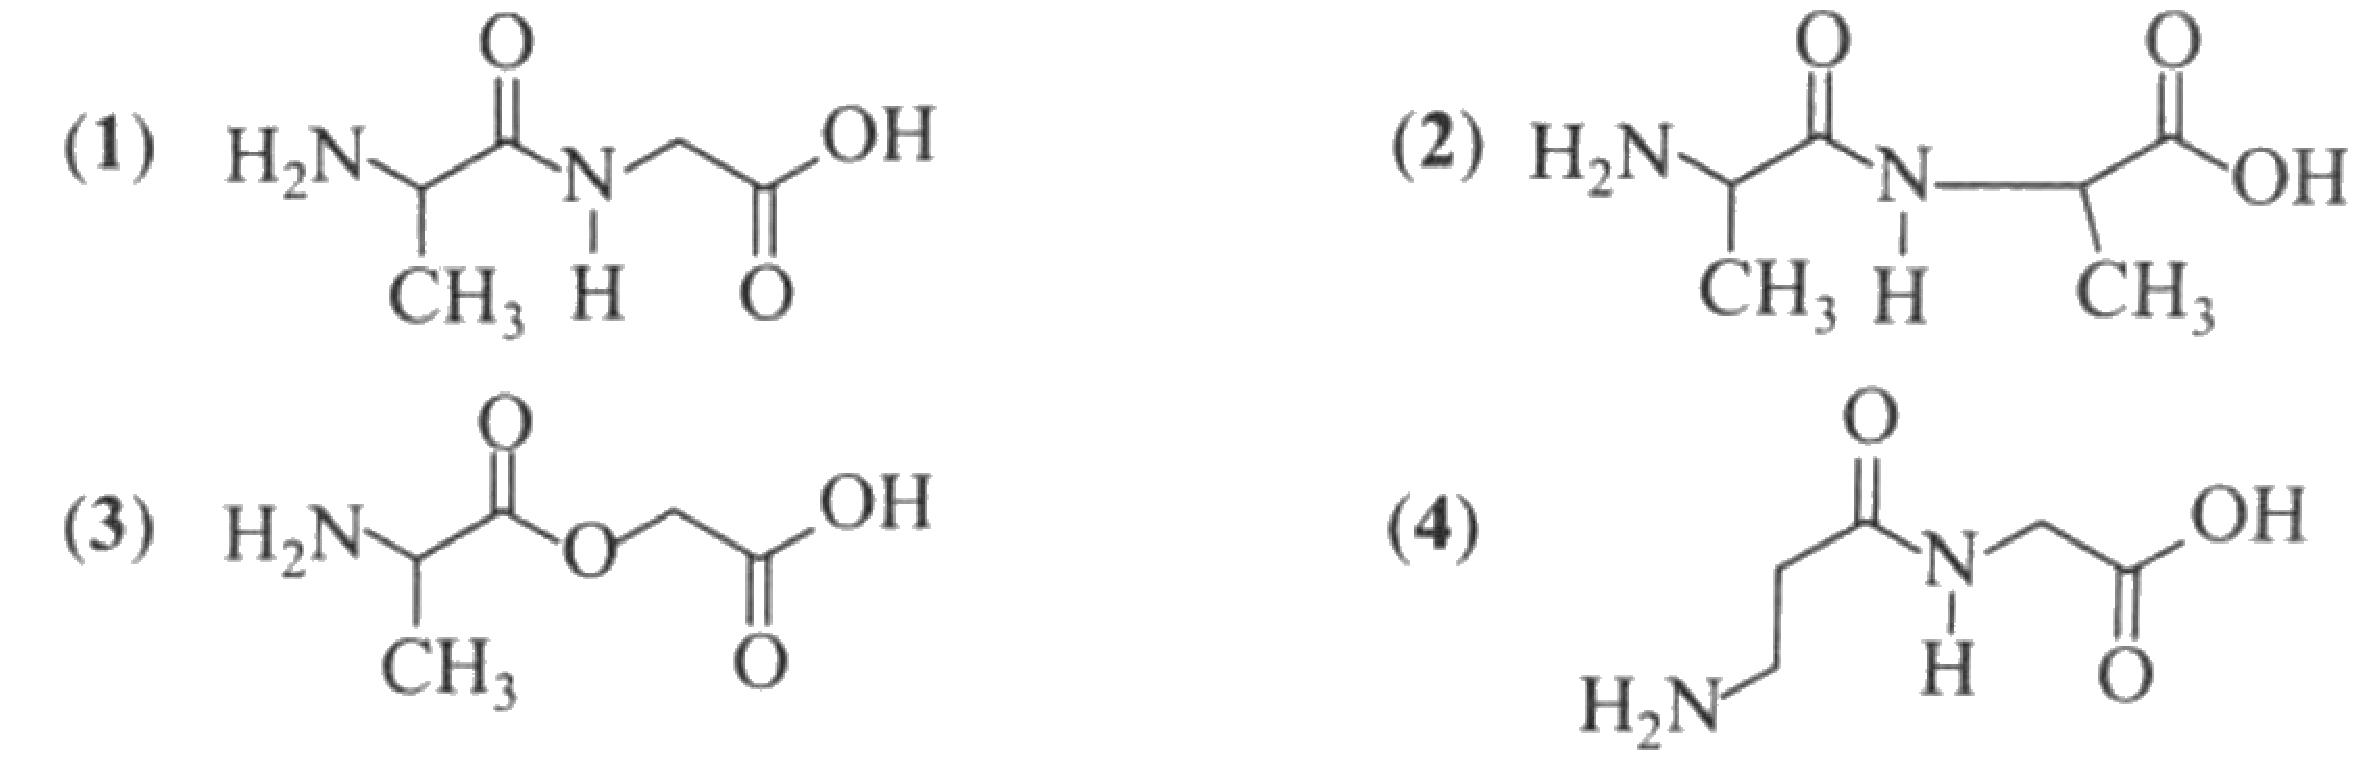
\includegraphics[width=9.5cm]{images_crop_de09/cau13_dipeptides.png}\par}
Trong các hợp chất trên, những hợp chất nào thuộc loại dipeptide?
\choice
{\True Hợp chất (1) và (2)}
{Hợp chất (1) và (3)}
{Hợp chất (2) và (3)}
{Hợp chất (2) và (4)}
\loigiai{
- Chất (1) cấu tạo từ Ala và Gly (đều là $\alpha$-amino acid) liên kết qua liên kết peptide => dipeptide Ala-Gly.\\
- Chất (2) cấu tạo từ 2 gốc Ala => dipeptide Ala-Ala.\\
- Chất (3) có liên kết ester -\ce{COO}-, không có liên kết peptide.\\
- Chất (4) có nhóm amino ở vị trí $\gamma$ (không phải $\alpha$-amino acid).\\
=> Các hợp chất thuộc loại dipeptide là (1) và (2).\\
\textbf{Chọn A.}}
\end{ex}

\begin{ex}
(SBT -- CĐ). Trong cấu trúc phân tử của chất cho ở hình bên, liên kết peptide là
{\centering
	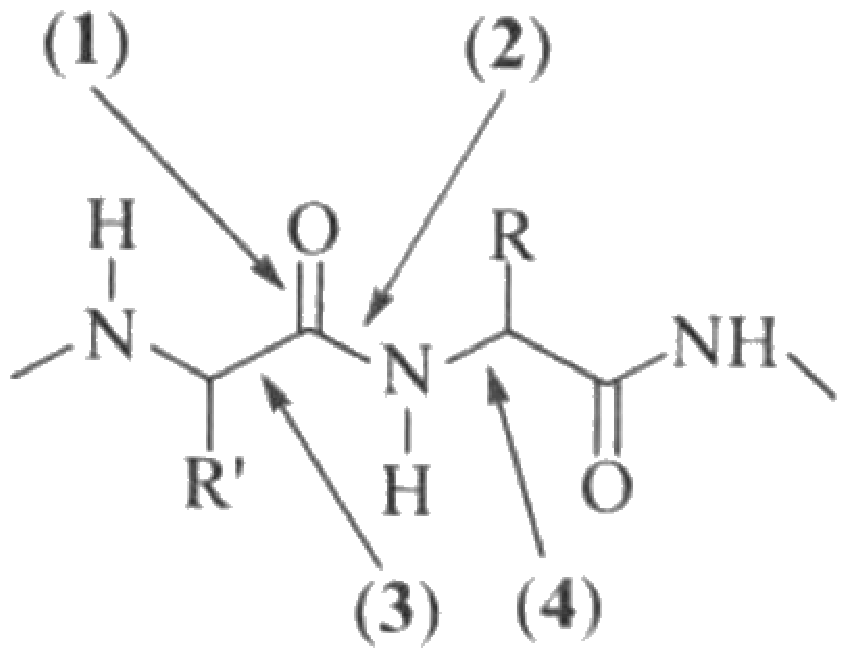
\includegraphics[width=4.5cm]{images_crop_de09/cau14_peptide_bond.png}\par}
\choice
{liên kết (1)}
{liên kết (3)}
{\True liên kết (2)}
{liên kết (4)}
\loigiai{
Liên kết peptide là liên kết amide -\ce{CO-NH}- giữa nhóm carboxyl của $\alpha$-amino acid này với nhóm amino của $\alpha$-amino acid khác. Trên hình vẽ, mũi tên (2) chỉ trực tiếp vào liên kết cộng hóa trị giữa C(\ce{=O}) và N(\ce{-H}).\\
\textbf{Chọn C.}}
\end{ex}

\begin{ex}
(SBT -- CTST). Loại dinh dưỡng nào sau đây \textbf{không} được cơ thể dự trữ để sử dụng?
\choice
{Tinh bột}
{Chất béo}
{\True Amino acid}
{Acid béo}
\loigiai{
Cơ thể có thể dự trữ glycogen (tinh bột động vật) và mỡ (lipid), nhưng không có cơ chế dự trữ amino acid tự do; amino acid dư thừa sẽ bị thoái hóa và thải ra ngoài.\\
\textbf{Chọn C.}}
\end{ex}

\begin{ex}
(SBT -- CĐ). Cho các hợp chất có công thức cấu tạo dưới đây:
{\centering
	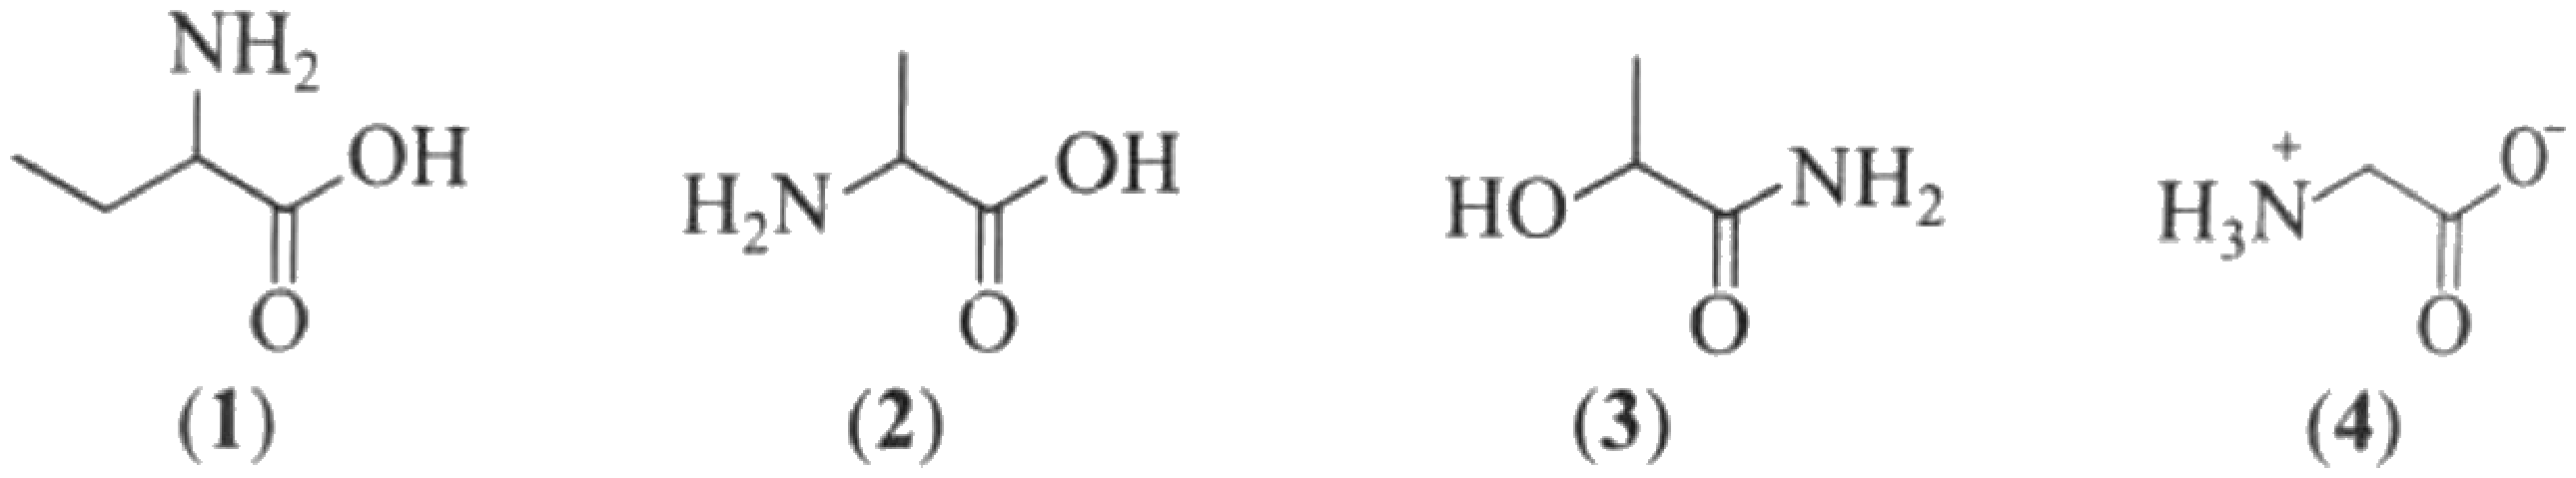
\includegraphics[width=10.0cm]{images_crop_de09/cau16_amino_acids.png}\par}
Những hợp chất nào trong số các chất trên thuộc loại $\alpha$-amino acid?
\choice
{Chất (2), chất (3) và chất (4)}
{Chất (1) và chất (2)}
{Chất (1) và chất (3)}
{\True Chất (1), chất (2) và chất (4)}
\loigiai{
$\alpha$-amino acid là hợp chất có nhóm amino (-\ce{NH2}) gắn trực tiếp vào carbon $\alpha$ (C2 liền kề -\ce{COOH}):\\
- Chất (1): 2-aminobutanoic acid => $\alpha$-amino acid.\\
- Chất (2): 2-aminopropanoic acid (alanine) => $\alpha$-amino acid.\\
- Chất (3): 2-hydroxypropanamide => hydroxy amide, không phải amino acid.\\
- Chất (4): $\ce{^+H3N-CH2-COO-}$ (glycine ion lưỡng cực) => $\alpha$-amino acid.\\
=> Các chất thuộc loại $\alpha$-amino acid là (1), (2) và (4).\\
\textbf{Chọn D.}}
\end{ex}

\begin{ex}
(SBT -- CĐ). Chất nào dưới đây \textbf{không} phải là amino acid?
\choice
{Lysine}
{Glycine}
{\True Aniline}
{Glutamic acid}
\loigiai{
Aniline (\ce{C6H5NH2}) là amine thơm, không có nhóm carboxyl (-\ce{COOH}) nên không phải amino acid.\\
\textbf{Chọn C.}}
\end{ex}

\begin{ex}
Cho các phát biểu sau:\\
(a) Sục khí \ce{CH3NH2} vào dung dịch \ce{FeCl3} có sinh ra kết tủa màu xanh.\\
(b) Không thể dùng quỳ tím để phân biệt ba dung dịch: alanine, lysine, glutamic acid.\\
(c) Dung dịch glutamic acid đổi màu quỳ tím thành xanh.\\
(d) Nhỏ vài giọt nước bromine vào dung dịch aniline thu được kết tủa đỏ nâu.\\
(e) Cho dung dịch HCl vào dung dịch glutamic acid thì không có phản ứng xảy ra.\\
(g) Methylamine có lực base yếu hơn ammonia.\\
Số phát biểu đúng là
\choice
{5}
{4}
{\True 0}
{3}
\loigiai{
(a) Sai, tạo kết tủa \ce{Fe(OH)3} màu nâu đỏ.\\
(b) Sai, dùng được quỳ tím để phân biệt cả 3 chất.\\
(c) Sai, glutamic acid làm quỳ tím hóa đỏ (hồng).\\
(d) Sai, aniline tạo kết tủa trắng 2,4,6-tribromoaniline.\\
(e) Sai, glutamic acid có nhóm -\ce{NH2} tác dụng với HCl.\\
(g) Sai, methylamine có lực base mạnh hơn ammonia.\\
=> Cả 6 phát biểu đều sai. Số phát biểu đúng là 0.\\
\textbf{Chọn C.}}
\end{ex}

\Closesolutionfile{ans}



\vspace{0.15cm}
\noindent
\textbf{PHẦN II (4,0 điểm -- 4 câu): Câu trắc nghiệm đúng sai.}\\
\textit{Thí sinh trả lời từ câu 1 đến câu 4. Trong mỗi ý a), b), c), d) ở mỗi câu, thí sinh chọn đúng hoặc sai.}

\setcounter{ex}{0}

\begin{ex}
(SBT -- KNTT). Các phát biểu về tính chất hoá học của dung dịch methylamine:
\choiceTF
{\True Phản ứng với HCl tạo thành \ce{CH3NH3Cl}}
{\True Hoà tan \ce{Cu(OH)2} tạo thành $\ce{[Cu(CH3NH2)4](OH)2}$}
{\True Phản ứng với \ce{FeCl3} tạo thành kết tủa \ce{Fe(OH)3}}
{\False Phản ứng với \ce{HNO2} tạo thành $\ce{CH3N2+}$}
\loigiai{
a) Đúng. $\ce{CH3NH2 + HCl -> CH3NH3Cl}$.\\
b) Đúng. Methylamine hòa tan \ce{Cu(OH)2} tạo phức chất xanh lam thẫm.\\
c) Đúng. $\ce{3CH3NH2 + FeCl3 + 3H2O -> Fe(OH)3 v + 3CH3NH3Cl}$.\\
d) Sai. Alkylamine phản ứng với \ce{HNO2} giải phóng khí \ce{N2} ngay ở nhiệt độ phòng: $\ce{CH3NH2 + HNO2 -> CH3OH + N2 ^ + H2O}$.\\
\textbf{Đáp án: a - Đ, b - Đ, c - Đ, d - S.}}
\end{ex}

\begin{ex}
(SBT -- CTST). Cho một số hợp chất chứa nguyên tố nitrogen như hình bên dưới:\\
{\centering
	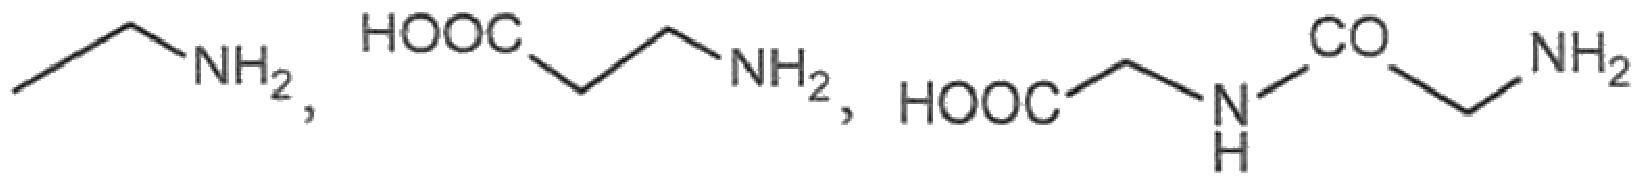
\includegraphics[width=9.5cm]{images_crop_de09/p2_cau2_compounds.png}\par}
Về tính chất vật lí của các chất, xét tính đúng/sai của các phát biểu sau:
\choiceTF
{\True Dễ tan trong nước}
{\False Ở điều kiện thường, có 1 chất là chất khí, 1 chất lỏng và 1 chất rắn}
{\True Chất có nhiệt độ nóng chảy thấp nhất là \ce{CH3CH2NH2}, cao nhất là \ce{HOOCCH2NHCOCH2NH2}}
{\True Khả năng tan tốt trong nước của các chất là do sự phân cực mạnh trong phân tử}
\loigiai{
a) Đúng. Cả 3 chất đều phân cực mạnh và tạo liên kết hydrogen với nước nên dễ tan trong nước.\\
b) Sai. Có 1 chất khí (ethylamine) và 2 chất rắn ($\beta$-alanine và Gly-Gly ion lưỡng cực), không có chất lỏng.\\
c) Đúng. Ethylamine là chất khí nên nhiệt độ nóng chảy thấp nhất; dipeptide Gly-Gly có phân tử khối lớn nhất và mạng tinh thể ion/hydrogen dày đặc nhất nên nhiệt độ nóng chảy cao nhất.\\
d) Đúng. Sự phân cực mạnh giúp các chất tan tốt trong dung môi phân cực như nước.\\
\textbf{Đáp án: a - Đ, b - S, c - Đ, d - Đ.}}
\end{ex}

\begin{ex}
Một peptide có cấu trúc như sau:
{\centering
	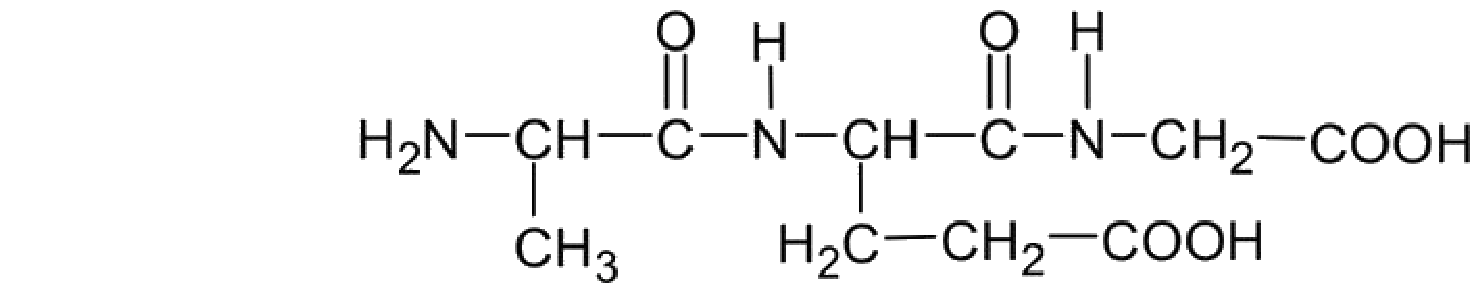
\includegraphics[width=8.5cm]{images_crop_de09/p2_cau3_tripeptide.png}\par}
\choiceTF
{\True Peptide trên chứa alanine, glutamic acid và glycine}
{\False Peptide trên có 3 liên kết peptide trong phân tử trên}
{\True Peptide trên có phản ứng màu biuret}
{\False Peptide trên là tetrapeptide}
\loigiai{
Peptide trên là tripeptide Ala-Glu-Gly.\\
a) Đúng. Cấu tạo từ 3 gốc amino acid: Ala, Glu và Gly.\\
b) Sai. Tripeptide chỉ có $3 - 1 = 2$ liên kết peptide (-\ce{CO-NH}-).\\
c) Đúng. Tripeptide trở lên cho phản ứng màu biuret tím với \ce{Cu(OH)2}.\\
d) Sai. Peptide được tạo từ 3 gốc amino acid nên là tripeptide.\\
\textbf{Đáp án: a - Đ, b - S, c - Đ, d - S.}}
\end{ex}

\begin{ex}
Bromelain và papain là những enzyme có tác dụng thuỷ phân protein. Bromelain có nhiều trong quả dứa (thơm). Bromelain được sử dụng để làm thuốc giảm sưng (viêm), điều trị viêm loét đại tràng\dots
{\centering
	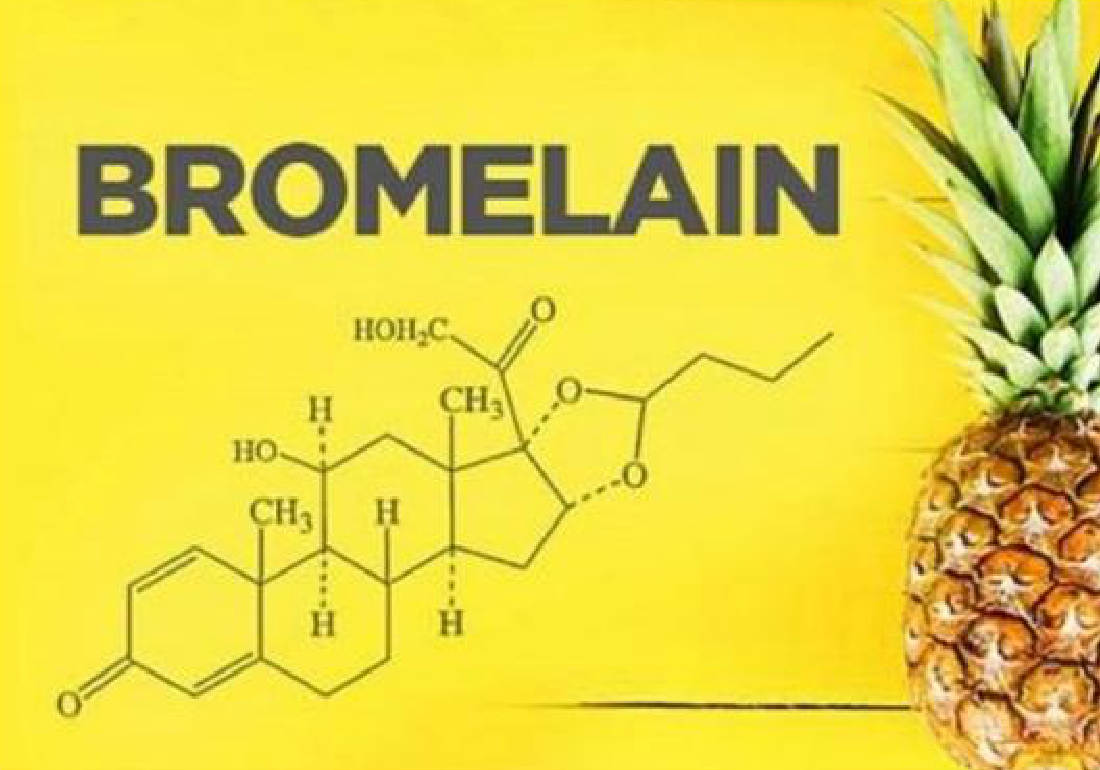
\includegraphics[width=6.0cm]{images_crop_de09/p2_cau4_bromelain.png}\par}
\choiceTF
{\True Thịt được ướp với nước ép dứa thì khi nấu sẽ nhanh mềm hơn}
{\True Do enzyme có nhiều trong quả dứa có tác dụng phân giải protein có trong thịt nên khiến cho thịt khi nấu cùng sẽ nhanh mềm hơn}
{\True Từ dứa có thể chiết xuất được Bromelain}
{\False Bromelain có chứa 7 nguyên tử oxygen}
\loigiai{
a) Đúng. Nước ép dứa chứa enzyme bromelain giúp làm mềm thịt hiệu quả.\\
b) Đúng. Enzyme bromelain xúc tác phản ứng thủy phân liên kết peptide trong thịt, làm mềm thịt nhanh khi nấu.\\
c) Đúng. Bromelain được chiết xuất từ thân và quả dứa.\\
d) Sai. Bromelain là một enzyme phức tạp bản chất là protein đại phân tử (chứa hàng trăm gốc amino acid), nên phân tử chứa hàng trăm đến hàng nghìn nguyên tử oxygen.\\
\textbf{Đáp án: a - Đ, b - Đ, c - Đ, d - S.}}
\end{ex}



\vspace{0.15cm}
\noindent
\textbf{PHẦN III (1,5 điểm -- 6 câu): Câu trắc nghiệm yêu cầu trả lời ngắn.}\\
\textit{Thí sinh trả lời từ câu 1 đến câu 6. Mỗi câu hỏi thí sinh điền câu trả lời vào ô tương ứng.}

\setcounter{ex}{0}

\begin{ex}
(SBT -- CTST). Các amine có tính base nên dễ phản ứng với dung dịch acid. Khi cho 1 mol methylenediamine phản ứng với dung dịch acid \ce{HCl} dư, số mol \ce{HCl} tham gia phản ứng là bao nhiêu?
\loigiai{
Methylenediamine có công thức là \ce{H2N-CH2-NH2}, chứa 2 nhóm chức amine bậc 1:\\
\centerline{$\ce{H2N-CH2-NH2 + 2HCl -> ClH3N-CH2-NH3Cl}$.}\\
Do đó 1 mol methylenediamine phản ứng với tối đa 2 mol \ce{HCl}.\\
\textbf{Đáp số: 2.}}
\end{ex}


\begin{ex}
Trong các dung dịch: \ce{CH3-CH2-NH2}, \ce{H2N-CH2-COOH}, \ce{H2N-CH2-CH(NH2)-COOH}, \ce{HOOC-CH2-CH2-CH(NH2)-COOH}, số dung dịch làm xanh quỳ tím là
\loigiai{
- \ce{CH3-CH2-NH2}: Amine có tính base => làm xanh quỳ tím.\\
- \ce{H2N-CH2-COOH} (Glycine: 1 \ce{NH2}, 1 \ce{COOH}) => không đổi màu quỳ tím.\\
- \ce{H2N-CH2-CH(NH2)-COOH} (2 \ce{NH2}, 1 \ce{COOH}) => tính base trội hơn => làm xanh quỳ tím.\\
- \ce{HOOC-CH2-CH2-CH(NH2)-COOH} (1 \ce{NH2}, 2 \ce{COOH}) => tính acid trội hơn => làm đỏ quỳ tím.\\
=> Có 2 dung dịch làm xanh quỳ tím.\\
\textbf{Đáp số: 2.}}
\end{ex}


\begin{ex}
(SBT -- CTST). Cho giá trị nhiệt độ nóng chảy ($^\circ$C) của glycine, trilaurin, \ce{H2O}, aniline, tristearin không theo thứ tự như sau: 0; $-6{,}0$; 46,5; 71,6; 262,0. Giá trị nào phù hợp với nhiệt độ nóng chảy của glycine?
\loigiai{
Glycine tồn tại ở dạng ion lưỡng cực $\ce{^+H3N-CH2-COO-}$ có mạng tinh thể ion với lực hút tĩnh điện rất mạnh nên có nhiệt độ nóng chảy cao nhất trong dãy, đạt $262{,}0\ ^\circ\text{C}$.\\
\textbf{Đáp số: 262.}}
\end{ex}


\begin{ex}
Cho một số hiện tượng thí nghiệm:\\
(1) Đun nóng dung dịch lòng trắng trứng thấy hiện tượng đông tụ lại, tách ra khỏi dung dịch.\\
(2) Trộn lẫn lòng trắng trứng, dung dịch \ce{NaOH} và một ít \ce{CuSO4} thấy xuất hiện màu đỏ gạch đặc trưng.\\
(3) Nhỏ vài giọt dung dịch \ce{HNO3} đặc vào dung dịch lòng trắng trứng thấy kết tủa màu vàng.\\
(4) Đốt cháy một mẫu lòng trắng trứng thấy xuất hiện mùi khét như mùi tóc cháy.\\
(5) Vắt chanh vào một cốc sữa, ta thấy hiện tượng đông tụ protein xuất hiện.\\
Có bao nhiêu hiện tượng thí nghiệm mô tả đúng?
\loigiai{
(1) Đúng, protein bị đông tụ bởi nhiệt độ.\\
(2) Sai, phản ứng màu biuret cho dung dịch phức chất màu tím đặc trưng.\\
(3) Đúng, phản ứng xanthoproteic cho kết tủa vàng.\\
(4) Đúng, đốt cháy protein có mùi khét đặc trưng.\\
(5) Đúng, acid citric làm đông tụ protein casein trong sữa.\\
=> Có 4 hiện tượng mô tả đúng: (1), (3), (4), (5).\\
\textbf{Đáp số: 4.}}
\end{ex}


\begin{ex}
Cho một loại protein chứa 3,2\% sulfur về khối lượng. Giả sử trong phân tử chỉ chứa 2 nguyên tử sulfur, phân tử khối của loại protein đó là bao nhiêu?
\loigiai{
Mỗi phân tử protein chứa 2 nguyên tử S, do đó khối lượng sulfur là $2 \times 32 = 64\ \text{amu}$.\\
Vì sulfur chiếm 3,2\% khối lượng phân tử protein:\\
$M = \dfrac{64 \times 100}{3{,}2} = 2000\ \text{amu}$.\\
\textbf{Đáp số: 2000.}}
\end{ex}


\begin{ex}
Thủy phân hoàn toàn 200 gam hỗn hợp gồm tơ tằm và lông cừu thu được 31,7 g glycine. Phần trăm khối lượng của glycine trong tơ tằm và lông cừu tương ứng là 43,6\% và 6,6\%. Thành phần phần trăm khối lượng tương ứng của tơ tằm trong hỗn hợp ban đầu là a\%. Xác định giá trị của a.
\loigiai{
Gọi khối lượng của tơ tằm và lông cừu trong hỗn hợp lần lượt là $x$ và $y$ (gam).\\
Ta có hệ phương trình:\\
$\begin{cases} x + y = 200 \\ 0{,}436x + 0{,}066y = 31{,}7 \end{cases} \implies \begin{cases} x = 50\ \text{g} \\ y = 150\ \text{g} \end{cases}$\\
Thành phần phần trăm khối lượng của tơ tằm trong hỗn hợp ban đầu là:\\
$a\% = \dfrac{50}{200} \times 100\% = 25\% \implies a = 25$.\\
\textbf{Đáp số: 25.}}
\end{ex}


\vspace{0.1cm}
\begin{center}
	\textbf{---------- HẾT ----------}
\end{center}

\vspace{0.3cm}
\noindent
\textbf{\large\color{mainGreen}BẢNG TỔNG HỢP ĐÁP ÁN ĐỀ SỐ 09}

\vspace{0.2cm}
\noindent\textbf{PHẦN I:}\\
\begin{tabular}{|c|c|c|c|c|c|c|c|c|c|c|c|c|c|c|c|c|c|}
\hline
\textbf{1} & \textbf{2} & \textbf{3} & \textbf{4} & \textbf{5} & \textbf{6} & \textbf{7} & \textbf{8} & \textbf{9} & \textbf{10} & \textbf{11} & \textbf{12} & \textbf{13} & \textbf{14} & \textbf{15} & \textbf{16} & \textbf{17} & \textbf{18} \\
\hline
A & C & A & C & A & D & C & D & B & B & B & A & A & C & C & D & C & C \\
\hline
\end{tabular}

\vspace{0.3cm}
\noindent\textbf{PHẦN II:}\\
\begin{tabular}{|c|c|c|c|c|}
\hline
\textbf{Câu} & \textbf{Lệnh hỏi a} & \textbf{Lệnh hỏi b} & \textbf{Lệnh hỏi c} & \textbf{Lệnh hỏi d} \\
\hline
\textbf{1} & Đ & Đ & Đ & S \\
\hline
\textbf{2} & Đ & S & Đ & Đ \\
\hline
\textbf{3} & Đ & S & Đ & S \\
\hline
\textbf{4} & Đ & Đ & Đ & S \\
\hline
\end{tabular}

\vspace{0.3cm}
\noindent\textbf{PHẦN III:}\\
\begin{tabular}{|c|c|c|c|c|c|c|}
\hline
\textbf{Câu} & \textbf{1} & \textbf{2} & \textbf{3} & \textbf{4} & \textbf{5} & \textbf{6} \\
\hline
\textbf{Đáp số} & 2 & 2 & 262 & 4 & 2000 & 25 \\
\hline
\end{tabular}

\end{document}
